\chapter{Task 1 - Multi-Robot Target Localization}
\label{ch:consensus}
In the last decade, the optimization community has developed a novel theoretical framework to solve optimization problems over networks of communicating agents. In this computational setting, agents (e.g., processors or robots) co-operate with the aim of optimizing a common performance index without resorting to a central computing unit. The key assumption is that each agent is aware of only a small part of the optimization problem, and can communicate only with a few neighbors.

In the so called Distributed Cost-Coupled Optimization Problem, the objective is to minimize the sum of $N$ local functions $\ell_i : \mathbb{R}^d \rightarrow \mathbb{R}$, each one depending on a common global variable $z \in Z \subseteq \mathbb{R}^d$: \\
\[\underset{z \in Z}{\min} \sum_{i=1}^N\ell_i(z)\]

% REWRITE
In this setup, robots usually update local solution estimates $z_i^k \in \mathbb{R}^d$ that eventually converge to a common optimal solution $z^* \in \mathbb{R}^d$. This setup is particularly suited for decision systems performing data analytics in which data are private and the consensus has to be reached on a common set of parameters characterizing a global classifier or estimator (e.g., neural network) based on all data. In cooperative robotics, this scenario can be interesting to reach a consensus on a common quantity, e.g., target estimation. Although Distributed Cost-Coupled Optimization provides the most general problem formulation; algorithms designed for such a framework require storing, sharing, and reaching consensus on a decision variable that includes the stack of all robots' estimates. \cite{TutorialOnDistributedOptimizationCooperativeRobotics} For this reason this is also called Consensus Optimization. 




% [ centralized ]
\paragraph{Centralized setting.}
In the centralized formulation of the problem, we assume access to the entire collection of cost functions $\ell_i(z)$ for $i = 1, \dots, N$, which allows us to define the global objective function as $\ell(z) = \sum_{i=1}^N \ell_i(z)$. A widely used method in this context is the Gradient Method, an iterative optimization algorithm whose update rule can be expressed as:
\begin{align*}
z^{k+1} &= z^k + \alpha^kd^k \\ 
        &= z^k - \alpha^k \nabla \ell(z^k),
\end{align*}
where $z^k$ denotes the current estimate of the optimal solution at iteration $k$, $\alpha^k$ is the step size (also referred to as the learning rate), $\nabla \ell(z^k)$ is the gradient of the global cost function at $z^k$ and $d^k=-\nabla \ell(z^k)$ is the steepest descent direction for minimizing the overall objective function.

% [ distributed ]
\paragraph{Distributed setting.}
In a distributed setting, each agent $i$ has access only to its local cost function $\ell_i(z)$ and communicates with a subset of other agents, typically those in its neighborhood. Instead of relying solely on local information, as in methods like the Incremental Gradient Method, distributed algorithms exploit inter-agent communication to improve convergence.

Figure \ref{fig:distributed_consensus_optimization} illustrates the evolution of local estimates $z_i^k$ and $z_j^k$. The agents iteratively update their estimates, which evolve over time within a two-dimensional cost landscape.

\begin{figure}[h!]
    \centering
    \begin{minipage}{0.55\linewidth}
        \centering
        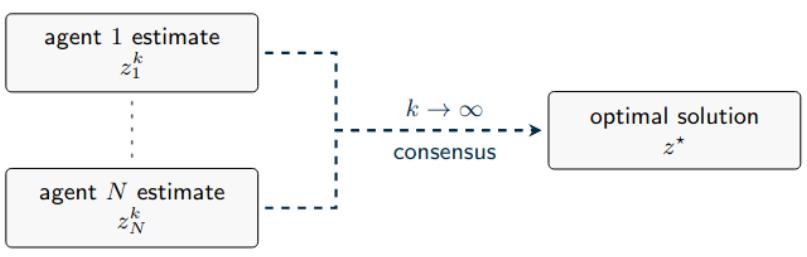
\includegraphics[width=\linewidth]{report/figs/consensus_optimization_1.jpg}
    \end{minipage}%
    \hfill
    \begin{minipage}{0.4\linewidth}
        \centering
        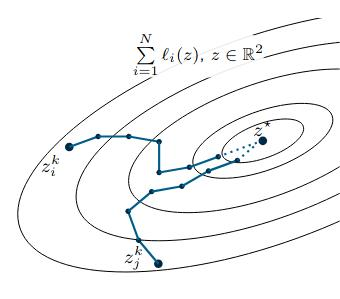
\includegraphics[width=\linewidth]{report/figs/consensus_optimization_2.jpg}
    \end{minipage}
    \caption{It shows the evolution of local estimates $z_i^k$ and $z_j^k$ in a distributed consensus optimization process. Through local communication and gradient updates, agents align their estimates over time and converge to the global optimum $z^*$ of the objective $\sum_{i=1}^N \ell_i(z)$, with $z \in \mathbb{R}^2$.}
    \label{fig:distributed_consensus_optimization}
\end{figure}

A typical update rule in a Distributed Gradient Method takes the form:
\begin{align*}
z_i^{k+1} = \left( \sum_{j \in N_i} a_{ij} z_j^k \right) - \alpha^k \nabla \ell_i\left( \sum_{j \in N_i} a_{ij} z_j^k \right),
\end{align*}

where $z_i^k$ is agent $i$'s estimate at iteration $k$, $N_i$ denotes the set of neighbors of agent $i$, and $a_{ij}$ are weights representing how much agent $i$ is getting influenced by the estimate of neighbor $j$. This formulation combines information from the neighborhood to approximate the global direction of descent.

However, the direction computed as $d_i^k = -\nabla \ell_i\left( \sum_{j \in N_i} a_{ij} z_j^k \right)$ does not correspond to the true gradient of the global function $\ell(z)$, as in the centralized case. Instead, it can be seen as an approximation that, on average, points toward the optimal solution. Due to this inaccuracy, especially near the optimum $z^*$, the method introduces a persistent error term, i.e. the estimate solution will ``walk" within a ball with radius depending on $\alpha$ instead of converging.

% [ alpha diminising ]
To mitigate this issue, a possible approach is to adopt a diminishing step size $\alpha^k$ that gradually decreases over the iterations and inhibits the second term. Under such conditions, it can be shown that the method converges asymptotically to the optimal solution.

% [ constant alpha ]
Using a constant stepsize $\alpha^k = \alpha > 0 \ \forall k$ not only simplifies the distributed implementation by removing the need for synchronization among agents on the iteration index or step value, but also can lead to improved convergence rates. Each agent can operate independently without global coordination, which is particularly beneficial in asynchronous or delay-prone networks, while still achieving faster convergence under suitable conditions.

% [ improve descent ]
To overcome the limitation of approximate convergence caused by the use of a constant stepsize, we aim to improve the local descent direction by reconstructing the true global gradient. Ideally, we would like each agent to compute a direction satisfying:
\[
d_i^k \xrightarrow[k \to \infty]{} -\frac{1}{N} \sum_{h=1}^{N} \nabla \ell_h(z_h^k),
\]
which corresponds to the average gradient of the global cost function. However, this quantity is not directly accessible in a distributed setting. For this reason we introduce a proxy variable that allows each agent to track the global gradient in a decentralized manner. We first introduce the core mechanism underlying this approach, and then show how it can be integrated into our specific setting.

% [ Dynamic Average Consensus ]
\paragraph{Dynamic Average Consensus.} 
\label{par:dynamic_avg}
The goal of the Dynamic Average Consensus (DAC) algorithm is to allow each agent to track, in a distributed manner, the time-varying average of local signals. Consider $N$ agents, each observing a time-varying local signal $r_i^k \in \mathbb{R}$ at time $k$. The global quantity of interest is the average:
\[
\bar{r}^k = \frac{1}{N} \sum_{i=1}^{N} r_i^k,
\]
which is not globally available due to the distributed nature of the system. Each agent maintains a local estimate $s_i^k$ and updates it via:
\[
s_i^{k+1} = \sum_{j \in N_i} a_{ij} s_j^k + \left( r_i^{k+1} - r_i^k \right),
\]
where the first term is a consensus step (a ``mixing" step, a weighted average over neighbors), and the second is a local innovation that incorporates changes in the observed signal.

Under the assumption that the signal variation is bounded, it can be shown that the tracking error remains bounded; in the special case where the signal variations vanish asymptotically, i.e., $\|r_i^{k+1} - r_i^k\| \to 0$, the algorithm guarantees perfect tracking:
\[
\lim_{k \to \infty} \|s_i^k - \bar{r}^k\| = 0.
\]

\medskip

% [ gradient tracking ]
The idea behind Gradient Tracking is to apply the dynamic average consensus mechanism to track the average gradient of the global objective function $\ell(z) = \sum_{i=1}^N \ell_i(z)$.

To this end, each agent uses its local gradient $\nabla \ell_i(z_i^k)$ as the input signal:
\[
r_i^k = \nabla \ell_i(z_i^k),
\]
and applies the update:
\[
s_i^{k+1} = \sum_{j \in N_i} a_{ij} s_j^k + \left( \nabla \ell_i(z_i^{k+1}) - \nabla \ell_i(z_i^k) \right), \quad s_i^0 = \nabla \ell_i(z_i^0).
\]
The descent direction at each agent is then set to:
\[
d_i^k = -s_i^k.
\]

If the gradient signals $\nabla \ell_i(z_i^k)$ converge (which is linked to the convergence of the decision variables $z_i^k$), the DAC mechanism ensures that each $s_i^k$ will converge to the true average gradient:
\[
s_i^k \xrightarrow[k \to \infty]{} \frac{1}{N} \sum_{h=1}^{N} \nabla \ell_h(z_h^k).
\]

This strategy enables each agent to approximate the centralized gradient direction in a fully distributed way, significantly improving the convergence properties compared to standard distributed gradient descent.

The Gradient Tracking algorithm reads as:
\begin{align*}
& z_i^{k+1} = \sum_{j \in N_i} a_{ij} z_j^k - \alpha s_i^k \\
& s_i^{k+1} = \sum_{j \in N_i} a_{ij} s_j^k + (\nabla \ell_i(z_i^{k+1}) - \nabla \ell_i(z_i^{k}))
\end{align*}

\paragraph{Gradient Tracking: Assumptions}
Let's make the following assumptions before providing the theorem results:
\begin{enumerate}
    \item $[\texttt{network}]$ Let $a_{ij}$ with $i,j \in \text{{1,..., N}}$ be non-negative entries of a weighted adjacency matrix A associated to the undirected and connected graph G, with $a_{ii} > 0$ and A doubly stochastic
    \item $[\texttt{cost}]$ For all $i \in \text{{1, ..., N}} $ each cost function $\ell_i : \mathbb{R}^d \rightarrow \mathbb{R}$ satisfies the following conditions:
    \begin{itemize}
        \item it is strongly convex with coefficient $\mu > 0$
        \item it has Lipschitz continuous gradient with constant $L > 0$
    \end{itemize}
\end{enumerate}

\paragraph{Gradient Tracking: Theorem}
Let Assumptions 1 and 2 hold true.
Then, there exists $\alpha^* > 0$ such that for all $\alpha \in (0, \alpha^*)$ the sequences of local solution estimates $\{z_i^k\}_{k\in\mathbb{N}}, \ i = 1, ..., N$, generated by the Gradient Tracking algorithm, asymptotically converge to a
(consensual) solution $z^*$ of the problem, i.e., for all $i = 1, ... , N$ , it holds:
\[ \lim_{k \to \infty} ||z_i^k - z^*|| = 0 \]

Moreover, the convergence rate is linear/the stability is exponential, i.e., for all $i = 1, ..., N$ there exists $\rho \in (0, 1)$ such that
\[ ||z_i^k - z^*|| \leq \rho ||z_i^{k-1} - z^*|| \leq \rho^k ||z_i^{0} - z^*|| \]
for all $k \in \mathbb{N}$.

\section{Distributed Consensus Optimization}
% [ DESCRIPTION OF THE TASK ]
We have implemented the Gradient Tracking algorithm as described, and verified its correctness through a set of simulations. In particular, we first tested the algorithm on a sum of quadratic functions, for which the optimal solution can be derived in closed form. This allowed us to compare the distributed solution with the centralized one and validate the convergence behavior.

In Task 1.2, we extended this analysis by comparing the performance of Gradient Tracking with the Centralized Gradient Method in the target localization scenario.
\paragraph{Assumption Checks.}
Certain structural properties of the communication graph are required to guarantee convergence of the distributed algorithm. In our setup, these assumptions are explicitly verified:

\begin{itemize}
    \item \textit{Aperiodicity}. The presence of self-loops in the graph ensures that it is aperiodic. From the perspective of distributed algorithms, this implies that each agent $i$ incorporates its own local information during each iteration.
    
    \item \textit{Strong connectivity}. We verified strong connectivity by computing the $N$-th power of the adjacency matrix $A$, where $N$ is the number of agents. The entry $(i, j)$ of $A^k$ indicates the existence of a path of length $k$ from node $i$ to node $j$. If all entries of $A^N$ are nonzero, this implies that every agent is reachable from every other agent within at most $N$ steps, confirming that the graph is strongly connected.
    
    \item \textit{Doubly stochastic weights}. The communication graph is generated as an undirected graph. Then, the weights are assigned according to the Metropolis-Hastings algorithm, which guarantees that the resulting weight matrix is doubly stochastic by construction.

    \item \textit{Cost function properties}. The cost functions must satisfy certain regularity conditions. Quadratic or quartic cost functions fulfill these assumptions and admit a unique global minimum.

\end{itemize}


% [ RESULTS (GRAPHS) ]
\begin{figure}[h!]
    \centering
    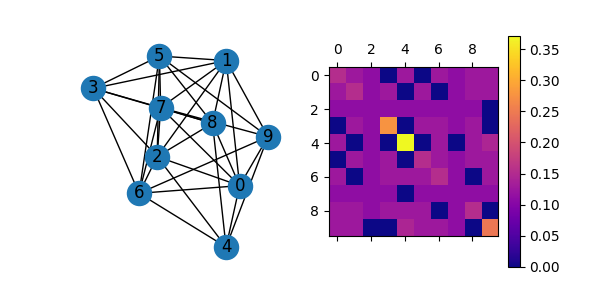
\includegraphics[width=0.45\linewidth]{report/figs/gradient_tracking_graph_1.png}
    \caption{Experiment 1: $N=10, \ \alpha=0.05$, $\texttt{GraphType.ERDOS\_RENYI} \text{ with } p=0.65$}
    \label{fig:gradient_tracking_graph}
\end{figure}

\paragraph{Experimental Results.}
As shown in Figure~\ref{fig:gradient_tracking_graph}, we report the results of a simulation using an Erd\H{o}s--R\'enyi communication graph with edge probability $p = 0.65$, $N = 10$ nodes, and Metropolis-Hastings weights for the adjacency matrix. The local cost functions are quadratic, of the form:
\[
\ell_i(z) = \frac{1}{2}z^\top Q_i z + r_i^\top z,
\]
where each $Q_i$ is a diagonal positive-definite matrix and $r_i$ is a randomly generated vector. The gradient is therefore given by $\nabla \ell_i(z) = Q_i z + r_i$.

The global optimum $z^*$ can be computed in closed form as:
\[
z^* = -\bar{Q}^{-1} \bar{r},
\]
where $\bar{Q} = \sum_{i=1}^N Q_i$ and $\bar{r} = \sum_{i=1}^N r_i$. In this specific configuration, the optimal cost is approximately $-3.262$.

\begin{figure}[h!]
    \centering
    \hspace*{-1.75cm}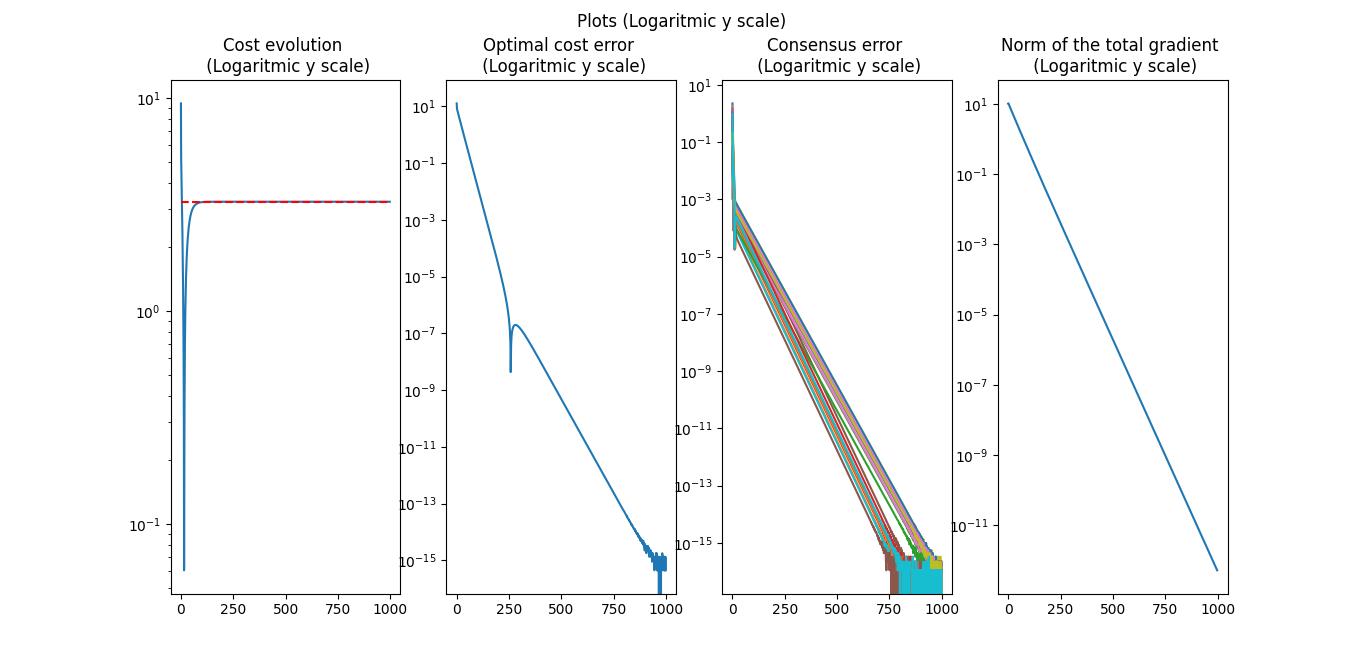
\includegraphics[width=1.25\linewidth]{report/figs/gradient_tracking_perf_1.png}
    \caption{Experiment 1: $N=10, \ \alpha=0.05$, $\texttt{GraphType.ERDOS\_RENYI} \text{ with } p=0.65$}
    \label{fig:gradient_tracking_perf}
\end{figure}

In the first plot (far left) of the Figure \ref{fig:gradient_tracking_perf}, we show the evolution of the absolute value of the cost function over time, in logarithmic scale. The cost starts from a positive value, then becomes negative, and finally stabilizes close to the optimal value (red dashed line).

The second plot displays the optimal cost error, defined as the difference between the current cost and the optimal one computed centrally. The convergence is linear, with the error rapidly decreasing to around $10^{-15}$ in $1000$ iterations.

The third plot shows the consensus error, defined as the distance between each local estimate $z_i^k$ and the average $\frac{1}{N} \sum_{j=1}^N z_j^k$. The consensus error of each agent converges to zero with a linear rate.

Finally, the fourth plot reports the norm of the total gradient. As expected, the gradient norm approaches zero, indicating that the algorithm has reached a stationary point. Due to the strong convexity of the cost functions, this stationary point also corresponds to the unique global optimum.


% [ BIRKHOFF VON NEUMANN ]
% As an alternative method for generating a communication graph, we used the Birkhoff-von Neumann theorem to construct a doubly stochastic matrix directly. Unlike the Metropolis-Hastings approach, which starts from a given graph topology and derives the weights accordingly, this method begins by generating a doubly stochastic matrix. The matrix is then interpreted as a weighted adjacency matrix, from which we extract the communication graph. The Birkhoff-von Neumann theorem states that any doubly stochastic matrix can be written as a convex combination of permutation matrices. Formally, for any doubly stochastic matrix $X \in \mathbb{R}^{n \times n}$, there exist permutation matrices $P_1, \dots, P_k$ and non-negative coefficients $\theta_1, \dots, \theta_k$ such that $\sum_{i=1}^k \theta_i = 1$ and:
% \[
% X = \theta_1 P_1 + \cdots + \theta_k P_k.
% \]
% This guarantees that the matrix lies within the convex hull of all $n \times n$ permutation matrices, providing a principled way to generate averaging matrices with desirable properties for distributed algorithms.

\section{Cooperative Multi-Robot Target Localization}
% [ DESCRIPTION OF THE TASK ]
As previously introduced, one relevant application of distributed optimization is cooperative target localization. Consider a team of $N \in \mathbb{N}$ mobile robots aiming to estimate the positions of one or more targets based on local, noisy measurements. As illustrated in Figure~\ref{fig:cooperative_localization_scenario}, each robot is equipped with sensors that allow it to observe the position of a target within a limited sensing range.

\begin{figure}[h!]
    \centering
    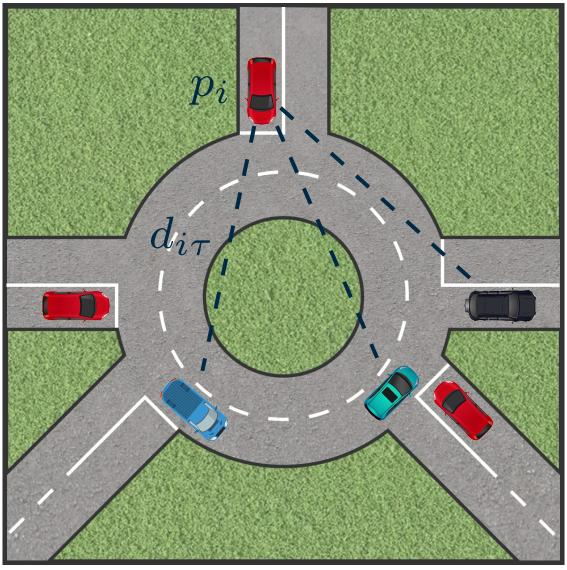
\includegraphics[width=0.45\linewidth]{report/figs/cooperative_localization_scenario.jpg}
    \caption{A team of red vehicles observing three targets (black, blue, and green vehicles). The blue, dashed lines represent the noisy measurements made one vehicle in the team.}
    \label{fig:cooperative_localization_scenario}
\end{figure}

In our simulation, we randomly generated $N$ robot positions, denoted by $p_i \in \mathbb{R}^d$, and $N_T \in \mathbb{N}$ target positions. For each robot $i$ and each target $\tau \in \{1, \ldots, N_T\}$, we computed the true Euclidean distance and then perturbed it by adding Gaussian noise with fixed mean $\mu$ and variance $\sigma^2$. This yielded a set of noisy measurements $d_{i\tau} \in \mathbb{R}_{\geq 0}$ representing the observed distance between robot $i$ and target $\tau$.

In this simplified scenario, we assume that each robot can measure its distance to every target.

% [ DEFINE $\ell_i$ ]
We define the local cost function for agent $i$ as:
\[
\ell_i(z) := \sum_{\tau=1}^{N_T} \left( d_{i\tau}^2 - \| z_\tau - p_i \|^2 \right)^2
\]
where $z = \mathrm{col}(z_1, \ldots, z_{N_T}) \in \mathbb{R}^{d N_T}$ is the optimization variable, i.e. the stacked vector of estimated target positions, with $\tau$-th block component $z_\tau \in \mathbb{R}^d$ representing the estimate for target $\tau$, and $p_i \in \mathbb{R}^d$ is the known position of robot $i$.

This is a least-squares formulation where each robot tries to minimize the difference between the squared distance measurement and the squared Euclidean distance between the estimated target and its own position.

\medskip

% [ GRADIENT COMPUTATION of the $\ell_i$ ]
\paragraph{Gradient computation of $\ell_i(z)$}
We observe that the function $\ell_i(z)$ is a sum of squared residuals, where each term only depends on the corresponding block variable $z_\tau$. We define the residual:
\[
r_{i\tau}(z_\tau) := d_{i\tau}^2 - \| z_\tau - p_i \|^2
\]
Then, the cost can be rewritten as:
\[
\ell_i(z) = \sum_{\tau=1}^{N_T} r_{i\tau}(z_\tau)^2
\]

We compute the gradient of $\ell_i$ with respect to each block $z_\tau \in \mathbb{R}^d$ using the chain rule:
\[
\nabla_{z_\tau}\ell_i(z) = 2 \cdot r_{i\tau}(z_\tau) \cdot \nabla_{z_\tau} r_{i\tau}(z_\tau)
\]

It remains to compute the gradient of the residual wrt. $z_\tau$:
\[
\nabla_{z_\tau} r_{i\tau}(z_\tau) = \nabla_{z_\tau} \left( d_{i\tau}^2 - \| z_\tau - p_i \|^2 \right) = -2(z_\tau - p_i)
\]

Therefore, we obtain:
\[
\nabla_{z_\tau} \ell_i(z) = -4 \left( d_{i\tau}^2 - \| z_\tau - p_i \|^2 \right) (z_\tau - p_i)
\]

\vspace{1em}

Finally, the full gradient $\nabla \ell_i(z) \in \mathbb{R}^{d N_T}$ is given by stacking the partial gradients for each target estimate:
\[
\nabla \ell_i(z) = 
\begin{bmatrix}
-4 \left( d_{i1}^2 - \| z_1 - p_i \|^2 \right)(z_1 - p_i) \\
-4 \left( d_{i2}^2 - \| z_2 - p_i \|^2 \right)(z_2 - p_i) \\
\vdots \\
-4 \left( d_{iN_T}^2 - \| z_{N_T} - p_i \|^2 \right)(z_{N_T} - p_i)
\end{bmatrix}
\]

\medskip

\paragraph{Simulations}
We begin by validating the correctness of our implementation using noise-free distance measurements.

In Figure \ref{fig:cooperative_localization_map}, the configuration for the subsequent simulations is illustrated. The map displays red dots that signify the agents, while the blue crosses indicate the target positions to be estimated. Both the positions of the agents and the positions of the targets are generated randomly within a world-size $10\times10$.

\begin{figure}[H]
    \centering
    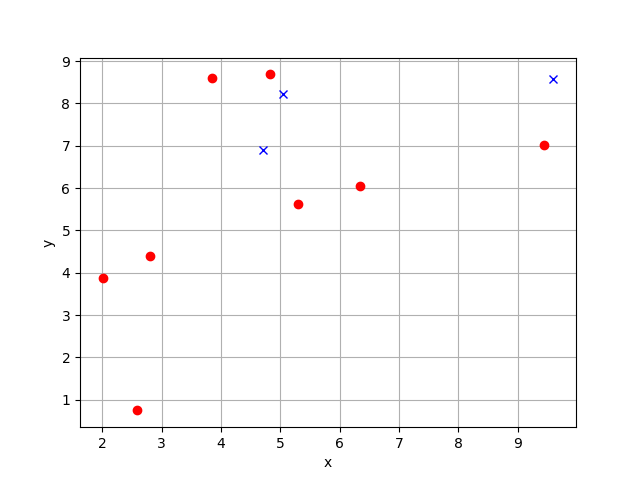
\includegraphics[width=0.5\linewidth]{report/figs/cooperative_localization_map.png}
    \caption{The map features red dots representing the agents and blue crosses indicating the target positions to be estimated.}
    \label{fig:cooperative_localization_map}
\end{figure}

\begin{figure}[H]
    \centering
    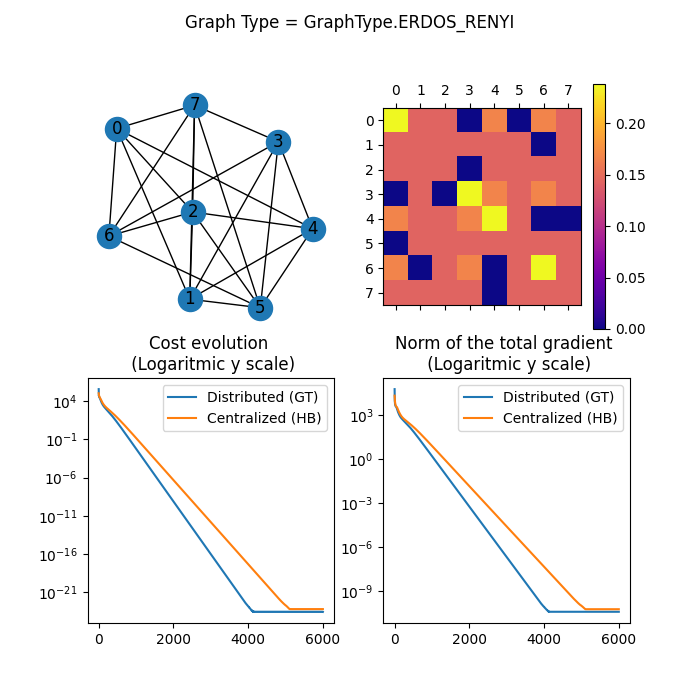
\includegraphics[width=0.45\linewidth]{report/figs/cooperative_localization_1_erdos.png}
    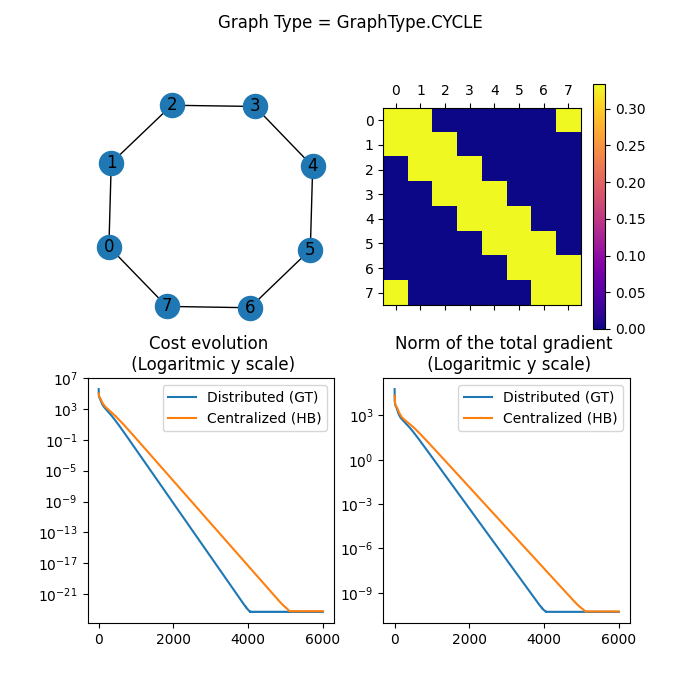
\includegraphics[width=0.45\linewidth]{report/figs/cooperative_localization_2_cycle.png}
    \caption{Comparison between two different communication topologies: \texttt{GraphType.ERDOS\_RENYI} and \texttt{GraphType.CYCLE}. Parameters used: $N = 8$ agents and $N_T = 3$ targets, with noise-free distances.}
    \label{fig:cooperative_localization}
\end{figure}

To validate the implementation, we tested the algorithm on different network topologies. In the plots shown in Figure \ref{fig:cooperative_localization}, we report two representative cases: one based on a randomly generated Erd\H{o}s--R\'enyi graph and the other on a cycle graph. In both cases, the cost function and the norm of the gradient converge to zero at a linear rate. Since the optimal value of the least-squares problem in the noise-free setting is zero, the decreasing cost confirms the correctness of the algorithm.

We now move to a more realistic scenario, where measurements are affected by Gaussian noise.
In the plots shown in Figure~\ref{fig:cooperative_localization_noisy}, we observe that the gradient norm converges to zero at a linear rate, while the cost function stabilizes at a value strictly greater than zero. This behavior is due to the presence of noise in the measurements, which prevents the cost from reaching the theoretical minimum.

\begin{figure}[H]
    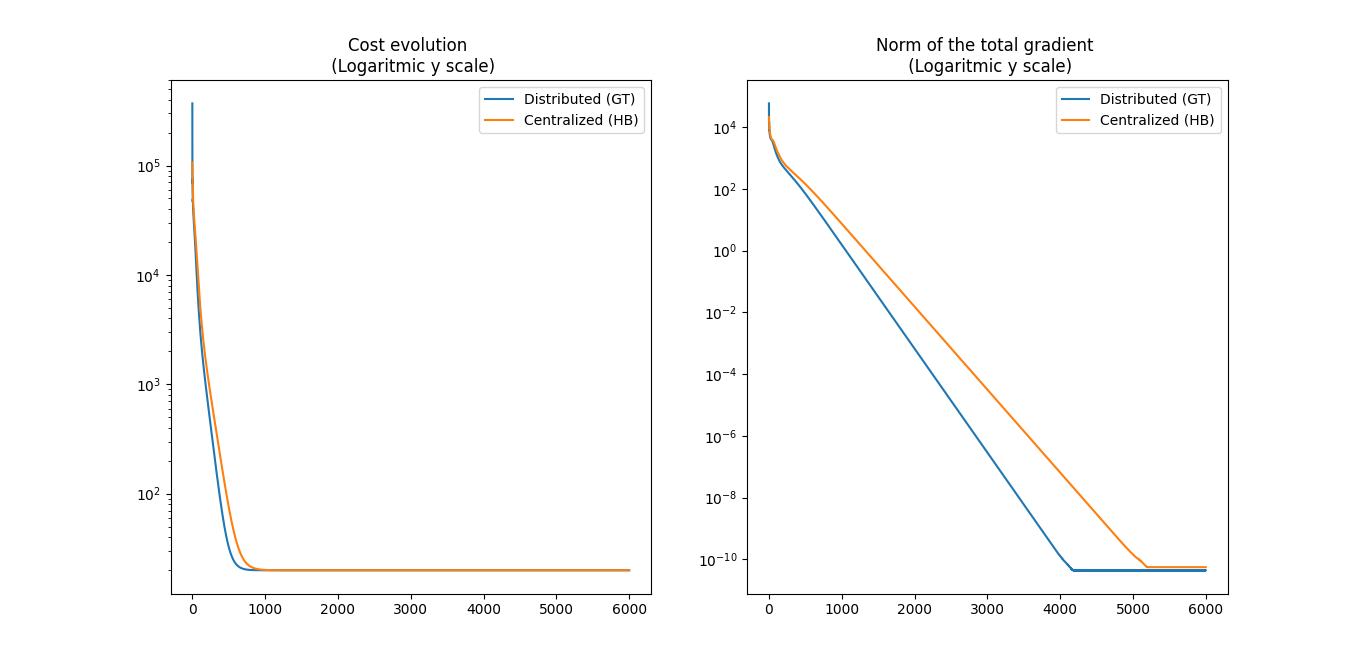
\includegraphics[width=0.5\linewidth]{report/figs/cooperative_localization_1_erdos_noisy.png}
    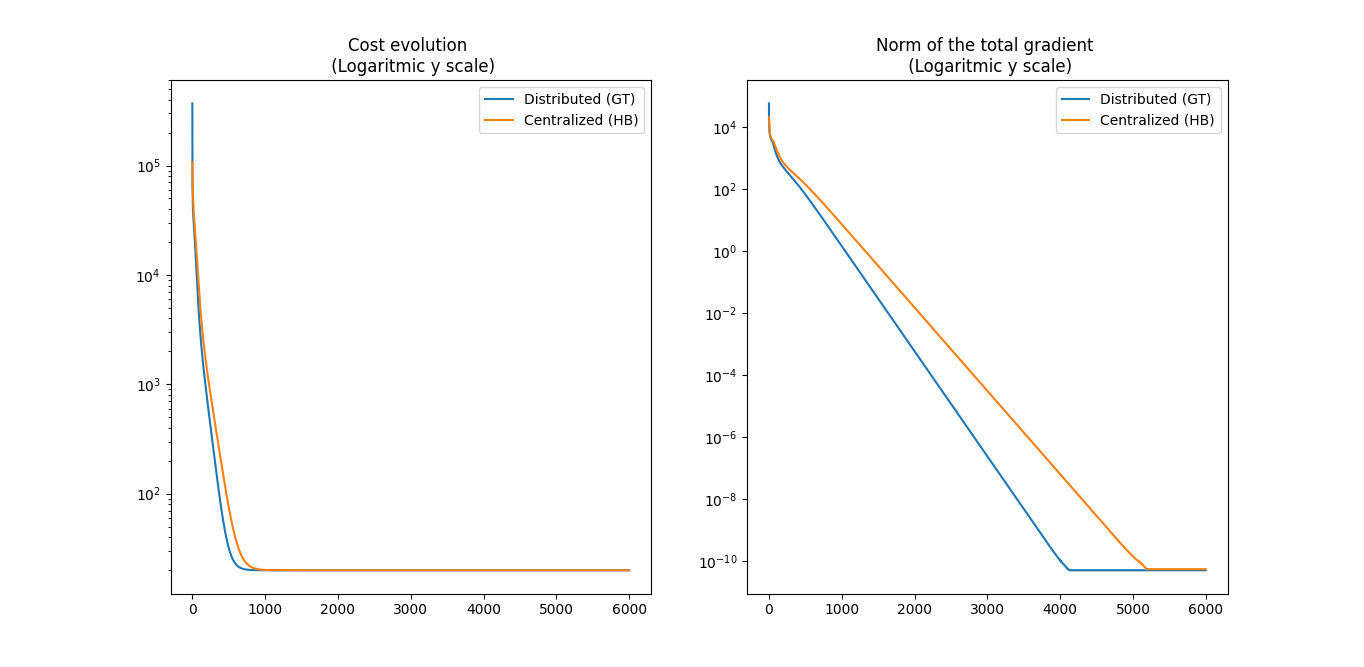
\includegraphics[width=0.5\linewidth]{report/figs/cooperative_localization_2_cycle_noisy.png}
     \caption{In this figure we can see two graph types respectively \texttt{GraphType.ERDOS\_RENYI} e \texttt{GraphType.CYCLE}. Parameters used: $N = 8$ agents and $N_T = 3$ targets, with noisy distances.}
     \label{fig:cooperative_localization_noisy}
\end{figure}



% Inoltre per aumentare il numero di agenti ma mantenere la feasibility, agenti non sovrapposti.
% {\color{red} per fare simulazioni realistiche con molti agenti FEISTEL}
